\chapter{Back to $\R^2$}

The bulk of the discussion thus far has focused on the one dimensional dynamics of the map $f_{c, \beta}$. The goal of this chapter is to briefly consider the implications of the one-dimensional results on the overall two-dimensional system. The results from the previous chapters pertain to finding parameter values which correspond to certain dynamical behaviors: superattracting periodic ($p_n)$, prezero ($z_n$), and homoclinic ($h_n$). It would be natural to look for corresponding features within the parameter space escape images of our family. We focus here on the parameter values which yield escaping critical orbits, namely the prezero parameter values, $z_n$.

Figure \ref{par} shows a zoom of the parameter space escape image for the map $f_{c,.001} = z^2 + c + \frac{.001}{\overline{z}^2}$. On top of this escape image we have overlaid some of the $z_n$ parameter values that are part of the sequence approaching $s_1^r$ from  the left. We can clearly see that along the $x$, or real, axis, there is a region of white corresponding to each of these parameter values. These white areas correspond to regions of escape, as we would expect: exactly along the real axis, the critical orbit is prezero which means that nearby points would also be drawn in toward zero and subsequently escape. In addition to the plotted $z_n$ values, it is also clear that there are many, many more escape regions along the real axis. These regions are a consequence of Proposition \ref{mainprop} which provides the infinite levels of parameter values causing escaping orbits. 


\begin{figure}[H]
	\centering
	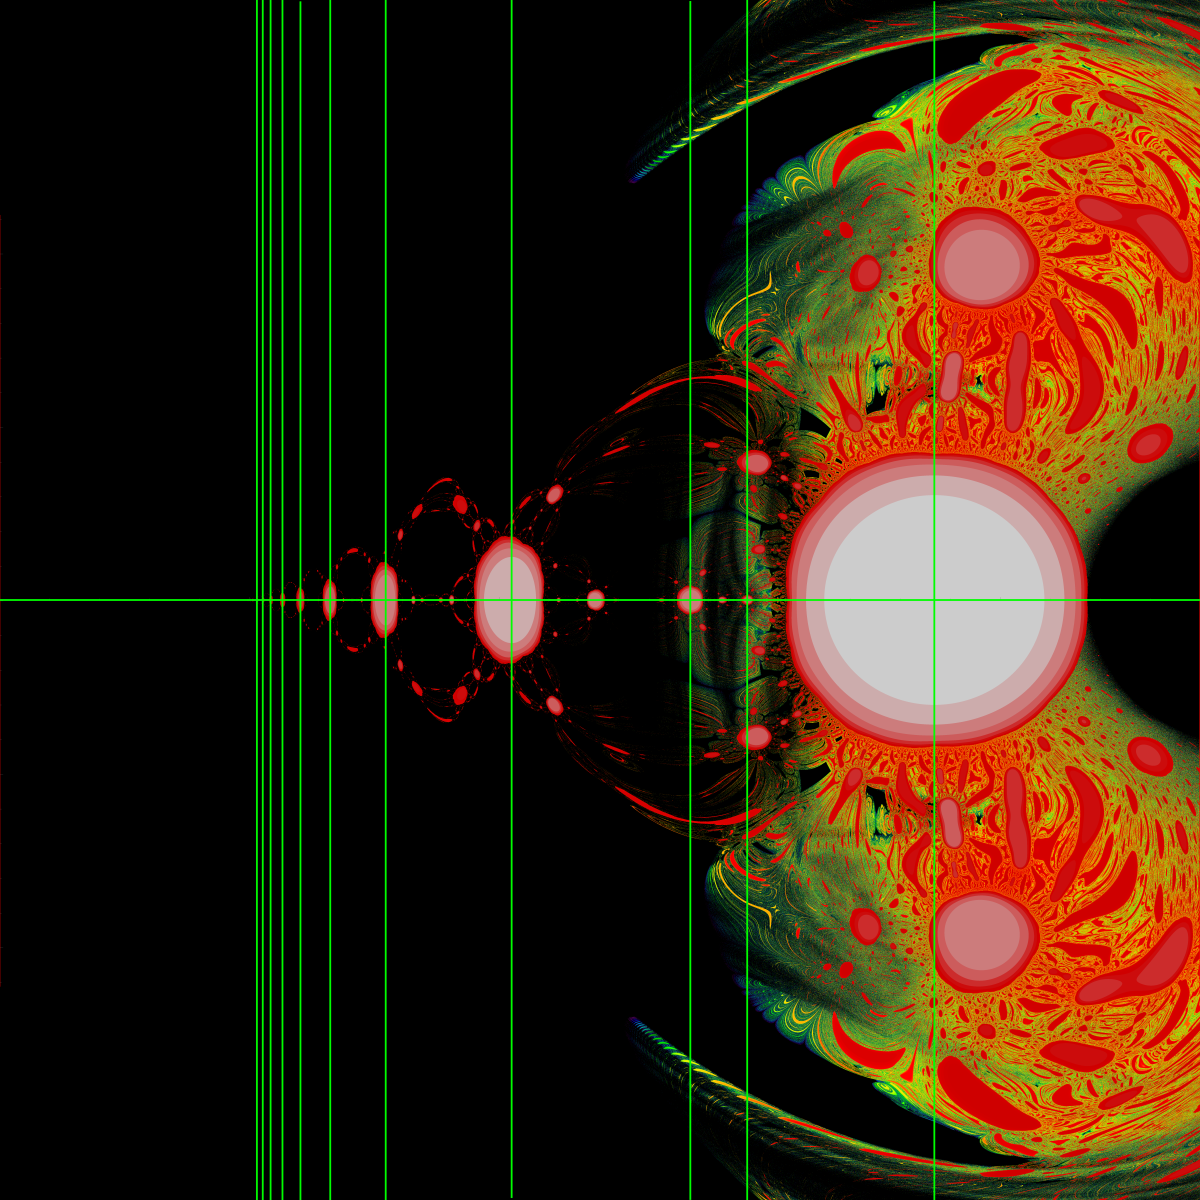
\includegraphics[width=.7\textwidth]{./img/par}
	\caption{Zoom of Figure \ref{perte} close to the real axis with the $z_n$ parameter values labeled with vertical green lines}
	\label{par}
\end{figure}

\begin{figure}[h]
	\centering
	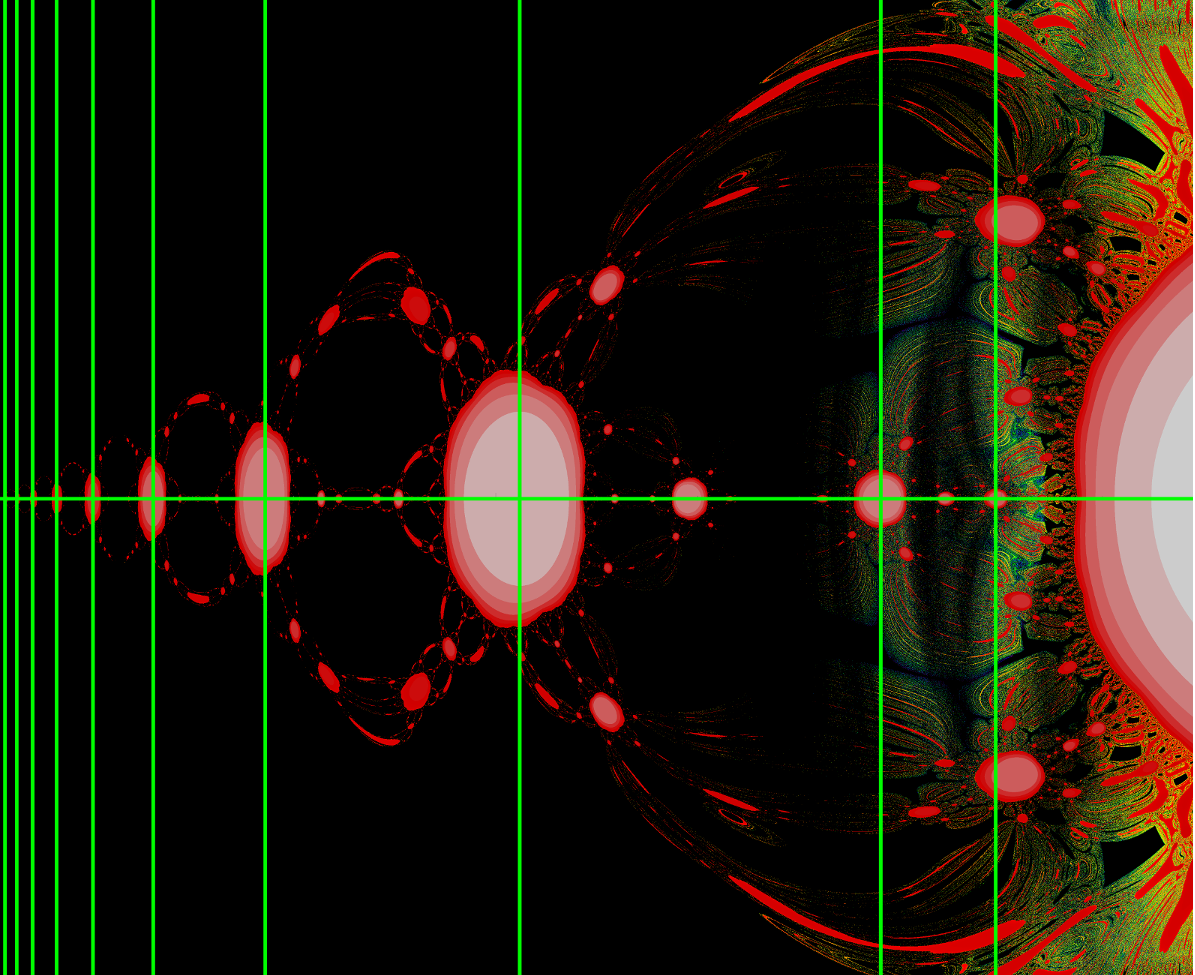
\includegraphics[width=.7\textwidth]{./img/zpar}
	\caption{A further zoom of Figure \ref{par} showing the accumulation of the $z_n$ parameter values}
	\label{zpar}
\end{figure}
\FloatBarrier